\documentclass[notes.tex]{subfiles}

\begin{document}

\chapter{Fundamentação teórica}

Este capítulo está organizado em 4 seções.
Na seção \ref{sec:def_graf} é apresentada a definição básica de grafo.
A seção \ref{sec:redes_complexas} define redes complexas e comunidades.
Na seção \ref{sec:propriedades_redes} aborda-se propriedades de redes complexas.
A seção \ref{sec:estado_arte} apresenta o estado da arte dos modelos de geração de redes complexas.

\section{Definição de grafos\label{sec:def_graf}}

Grafos podem trivialmente ser definidos como $\G = (\V, \E)$ onde $\V$ é um conjunto dos vértices de  $\G$ e  $\E$ é um conjunto de pares não ordenados de vértices adjacentes em $\G$, i.e. as arestas.

\begin{figure}[htpb]
    \centering
    \caption{Exemplo de grafo}\label{fig:graph_example}
    \fbox{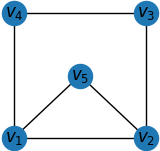
\includegraphics[width=0.4\textwidth]{figures/graph_example.png}}
    \fonte{elaborado pelo autor.}
\end{figure}

No exemplo da \autoref{fig:graph_example}, pode se representar o mesmo grafo com $\V = \{v_1, v_2, v_3, v_4, v_5\}$ e $\E = \{\{v_1, v_2\}, \{v_2, v_3\}, \{v_3, v_4\}, \{v_4, v_1\}, \{v_1, v_5\}, \{v_2, v_5\}\}$.
Dentro desse grafo, o subgrafo formato pelos vértices $v_1$, $v_2$ e $v_5$ é também um grafo completo.
A esse conjunto de vértices que forma um subgrafo completo dá-se o nome de clique \cite{fortunato2010community}.

Variações dessa definição incluem dígrafos, isso é, grafos direcionados, onde as arestas são pares ordenados.
Alternativamente, é possível a utilização de triplas para definir pares de vértices adjacentes, com um peso para essa aresta.
Grafos onde encontram-se auto referências (arestas ligando um vértice a ele mesmo) ou arestas paralelas (onde um par de vértices está ligado por mais de uma aresta) são chamados de multígrafos.

\section{Redes complexas e comunidades\label{sec:redes_complexas}}

A definição de clique pode ser utilizada como um ponto de partida para conceito de comunidade, partindo de uma perspectiva local \cite{fortunato2010community}.
É facilmente observável, no entanto, que essa é uma definição muito limitante de comunidade, é raro que comunidades de pessoas apresentem tanta homogeneidade a ponto de todos os membros conhecerem todos os outros membros.
De fato, \citeonline{fortunato2010community} indica que a definição do que é uma comunidade varia de acordo também com o contexto de estudo, mas que algumas características são universais.
Uma comunidade, dentro de qualquer definição, deve ser um sub grafo conexo, por exemplo \cite{fortunato2010community}. 

\citeonline{largeron2015generating} definem comunidade como uma classe de estrutura topológica comum a redes complexas, essas comunidades são categorizadas por terem uma densidade de vértices elevada.
\citeonline{shen2009detect} entendem que comunidades sejam estruturas que contenham múltiplos cliques dentro de si, e que essas comunidades se dispões em uma estrutura recursiva.
\citeonline{akoglu2009rtg} descrevem comunidades como estruturas modulares, onde nodos de um vértice formam grupos distintos entre si por que os membros do grupo tem maior chance de estarem conectados entre si do que estarem conectar com membros de outros grupos.
\citeonline{girvan2002community} definem ``Cluster'' e comunidade como duas propriedades distintas, o primeiro sendo a probabilidade de dois nodos ambos adjacentes a um terceiro serem também adjacentes entre si, e a segunda como sendo condutos de vértices densamente conectados entre si, e esparsamente conectados para além de si.

As definições são agrupadas em três classes distintas por \citeonline{fortunato2010community}: definição local; definição global; e definição por similaridade de vértice.
Essas definições não são mutuamente exclusivas, mas também não são ortogonais uma a outra.
Segundo \citeonline{fortunato2010community}, a definição local parte das características topológicas internas à comunidade.
Nominalmente, isso significa a existência de um conjunto considerável de arestas internas a comunidade e um conjunto limitado de arestas para além da comunidade.

A definição global de comunidades é aplicada aos casos onde a presença de clusters é uma característica inerente ao grafo ao qual se está estudando \citeonline{fortunato2010community}.
Essa propriedade inerente ao grafo pode ser definida como alguma propriedade dos vértices do objeto em questão e que partindo disso se atribui pertencimento a comunidades, ou ainda por comparação com um exemplo nulo \citeonline{fortunato2010community}.
No caso de comparação com um exemplo nulo, define-se uma comunidade pela característica de uma não ser presente dentro do que é chamado de ``grafo aleatório'' \cite{fortunato2010community}.
Essa definição de um modelo nulo é crucial para o trabalho de \citeonline{girvan2002community}, o modelo nulo considerado é um modelo de um grafo construído a partir do grafo original onde os vértices tem o mesmo grau, mas a probabilidade de dois vértices estarem ligados é constante independente de quais os vértices.

A definição de comunidade por similaridade de vértice se baseia na tendência de que em muitas aplicações, membros de comunidades são mais similares entre si do que seria esperado de um conjunto do mesmo tamanho escolhido aleatoriamente \cite{fortunato2010community}.
Essa definição se faz visível nos trabalhos de \citeonline{akoglu2009rtg} e de \citeonline{largeron2015generating}.
Na observação desses dois trabalhos também é interessante o questionamento de como se define semelhança, \citeonline{akoglu2009rtg} representam os vértices como sequencias de caracteres de tamanhos variáveis em que a probabilidade de dois vértices estarem ligados é maior conforme mais caracteres eles compartilham; e \citeonline{largeron2015generating} representam os vértices como pontos em um espaço $n$-dimensional e definem que vértices são mais semelhantes quando a distância euclideana deles é menor.

Também independente de qual definição de comunidade que se esteja utilizando, existem os conceitos de partição e cobertura.
Segundo \citeonline{fortunato2010community}, uma partição é uma divisão dos vértices de um grafo tal que cada vértice pertença a um e exatamente um cluster.
O caso de um vértice ``livre'', não pertencendo a nenhuma comunidade, é trivialmente resolvido incluindo ele a comunidade com a qual ele tem mais adjacências.
Mas o caso de vértices que pertençam a mais de uma comunidade, i.e. comunidade que se sobreponham, é mais interessante.
\citeonline{fortunato2010community} define uma cobertura como uma divisão dos vértices em clusters onde cada vértice pertence a um ou mais clusters.
\citeonline{fortunato2010community} também descreve o conceito de comunidades hierárquicas, como sendo comunidades cuja estrutura interna também se organiza em clusters de escala menor do que o original.

\citeonline{fortunato2010community} oferece também o conceito de ``função de qualidade'', sendo uma função que mapeia uma partição para um espaço de comparação, usualmente em números reais, onde partições que mapeiem para valores maiores são consideradas melhores.
Segundo \citeonline{fortunato2010community} função de qualidade mais comumente utilizada é a modularidade $Q$ de \citeonline{girvan2002community}.

\begin{equation}\label{eq:mod}
    Q = \frac{1}{2m}\sum_{ij}\Bigg(A_{ij}-\frac{K_iK_j}{2m}\Bigg)\delta(C_i, C_j)
\end{equation}

Essa função no entanto não se aplica adequadamente ao caso de comunidades sobrepostas ou comunidades hierárquicas, para tanto, é necessário utilizar a função de modularidade estendida, conforme desenvolvido por \citeonline{shen2009detect}.

\begin{equation}\label{eq:mod_e}
    EQ = \frac{1}{2m}\sum_{i}\sum_{v \in C_i, w \in C_i}\frac{1}{O_vO_w}\Bigg[A_{vw} - \frac{K_vK_w}{2m} \Bigg]
\end{equation}

Tanto no caso da fórmula da equação \ref{eq:mod} quanto no da \ref{eq:mod_e} a função definida é uma somatória em que alguns termos se repetem.
Primeiramente, é preciso descrever que a função $\delta(C_iC_j)$ retorna um se $C_i$ for igual a  $C_j$, e zero em outro caso \cite{fortunato2010community}.
Considerando isso, no caso de uma partição (sem comunidades hierárquicas, e sem comunidades sobrepostas), as duas somatórias iteram sobre os mesmos valores, a primeira com os vértices $i$ e $j$ e a segunda com os vértices $v$ e  $w$.

Essa iteração olha para todos os pares de vértices que compartilham alguma comunidade, e soma o valor de $A_{ij}$, sendo $A$ a tabela de adjacência do grafo em questão.
Então é subtraído um valor $\sfrac{K_iK_j}{2m}$, onde  $K_i$ é o grau do vértice $i$ e  $m$ é a quantidade de arestas no grafo ($2m$ portanto é a soma dos graus de todos os vértices).
Esse valor é a probabilidade de uma aresta entre os vértices  $i$ e  $j$ no modelo nulo de \citeonline{girvan2002community}, considerando que os graus se mantém mas que a probabilidade da presença de uma aresta é uniforme.

A fórmula $EQ$ de \citeonline{shen2009detect} contém também o termo escalar $\sfrac{1}{O_vO_w}$.
Nesse caso, o valor $O_i$ é a quantidade de comunidades a qual pertence o vértice $i$.
Isso permite a aplicação da modularidade estendida para os casos de grafos com comunidades sobrepostas.
Vértices que estejam em duas comunidades contribuirão para a modularidade a partir das duas, mas tendo a magnitude da sua contribuição escalada a metade.

\section{Propriedades de redes complexas\label{sec:propriedades_redes}}

Além de estruturas topológicas que podem ser denominas comunidades, redes complexas tem algumas propriedades topológicas bastante comuns e relevantes.
Algumas delas são: mundo pequeno; anexação preferencial; liberdade de escala; e homofilia.

\subsection{Mundo pequeno, Anexação preferencial e Liberdade de escala}

\citeonline{largeron2015generating} descrevem a propriedade de mundo pequeno como a característica de um sistema de ter um diâmetro logaritmicamente proporcional a quantidade de vértices em um grafo.
Isso é, a distância entre os dois vértices que estão a mais arestas de distância, denominada diâmetro, cresce logaritmicamente conforme observa-se exemplos maiores de grafos do sistema.
Essa propriedade implica que em sistemas bastante grandes, é preciso uma quantidade relativamente pequena de saltos de nodo a nodo para se atingir qualquer membro do grafo.
Essas propriedades serão exploradas a diante.

\citeonline{largeron2015generating} definem a anexação preferencial como uma propriedade de um sistema em que vértices tendem a se ligar com outros vértices que sejam parecidos e que tenham grau elevado.
A implicação é que dado um sistema onde se vai adicionar um vértice, a maior parte das arestas desse novo vértice devem ligá-lo a outro com grau igual ou maior do que o próprio.

Para atingir essa distribuição característica, o modelo de \citeonline{slota2019scalable} fazem com que os vértices se dividam em diferentes escalas, de forma que os vértices de uma escala se liguem apenas entre si e com os membros das escalas imediatamente vizinhas.
De grafos com essa distribuição onde o grau relativo de dois vértices adjacentes tende a não apresentar saltos demasiadamente grandes, se diz que são livres de escala \cite{largeron2015generating}.

\subsection{Cluster e comunidades}

\citeonline{girvan2002community} diferenciam explicitamente entre a definição de clusters e de comunidades.
Os autores apontam um cluster como sendo um triângulo, em outras palavras, um subgrafo completo com três vértices.
Essa definição aparentemente arbitrária é relevante no entendimento do coeficiente de clusterização, definido como a proporção de quantas triplas conexas são triângulos.


\begin{equation}\label{eq:coef_clus}
    C = \frac{3 \times (\text{número de triângulos do grafo})}{(\text{número de triplas conexas do grafo})}
\end{equation}


A conceitualização de um cluster é relevante dentro do estudo de redes complexas na medida em que a implicação é de dois vértices serem ligados por compartilharem uma relação com um terceiro.
O coeficiente $C$ sendo igual a 1 implica que o grafo é um grafo completo \cite{girvan2002community}.
Mais que isso, esse coeficiente, dado um vértice, é a probabilidade de quaisquer dois vértices adjacentes a ele serem adjacentes entre si.

\subsection{Homofilia e Homogeneidade de comunidades}

Homofilia é a tendência em um sistema de que dois vértices conectados sejam semelhantes entre si \cite{akoglu2009rtg}.
Essa propriedade está intimamente ligada a definição de comunidade por semelhança de vértices.
Essa definição de semelhança é deliberadamente vaga, pois dentro de sistemas distintos é trivial imaginar funções de semelhança distintas.
Observa-se que em grafos obtidos em sistemas do mundo real, a topografia otimiza alguma função de forma aos vértices serem mais parecidos com os vértices aos quais são adjacentes \cite{largeron2015generating}.

Homofilia como propriedade é intimamente ligada a uma outra característica que se observa de grafos do mundo real, em diferentes aplicações as comunidades tendem a ser mais homogêneas do que o grafo ao qual pertencem \cite{largeron2015generating}.
Pode-se afirmar que um grafo onde isso ocorra tem a propriedade de ``comunidades homogêneas''.

\begin{figure}[htpb]
    \centering
    \caption{Exemplo de grafo com comunidades hierárquicas}\label{fig:graph_hier_com}
    \fbox{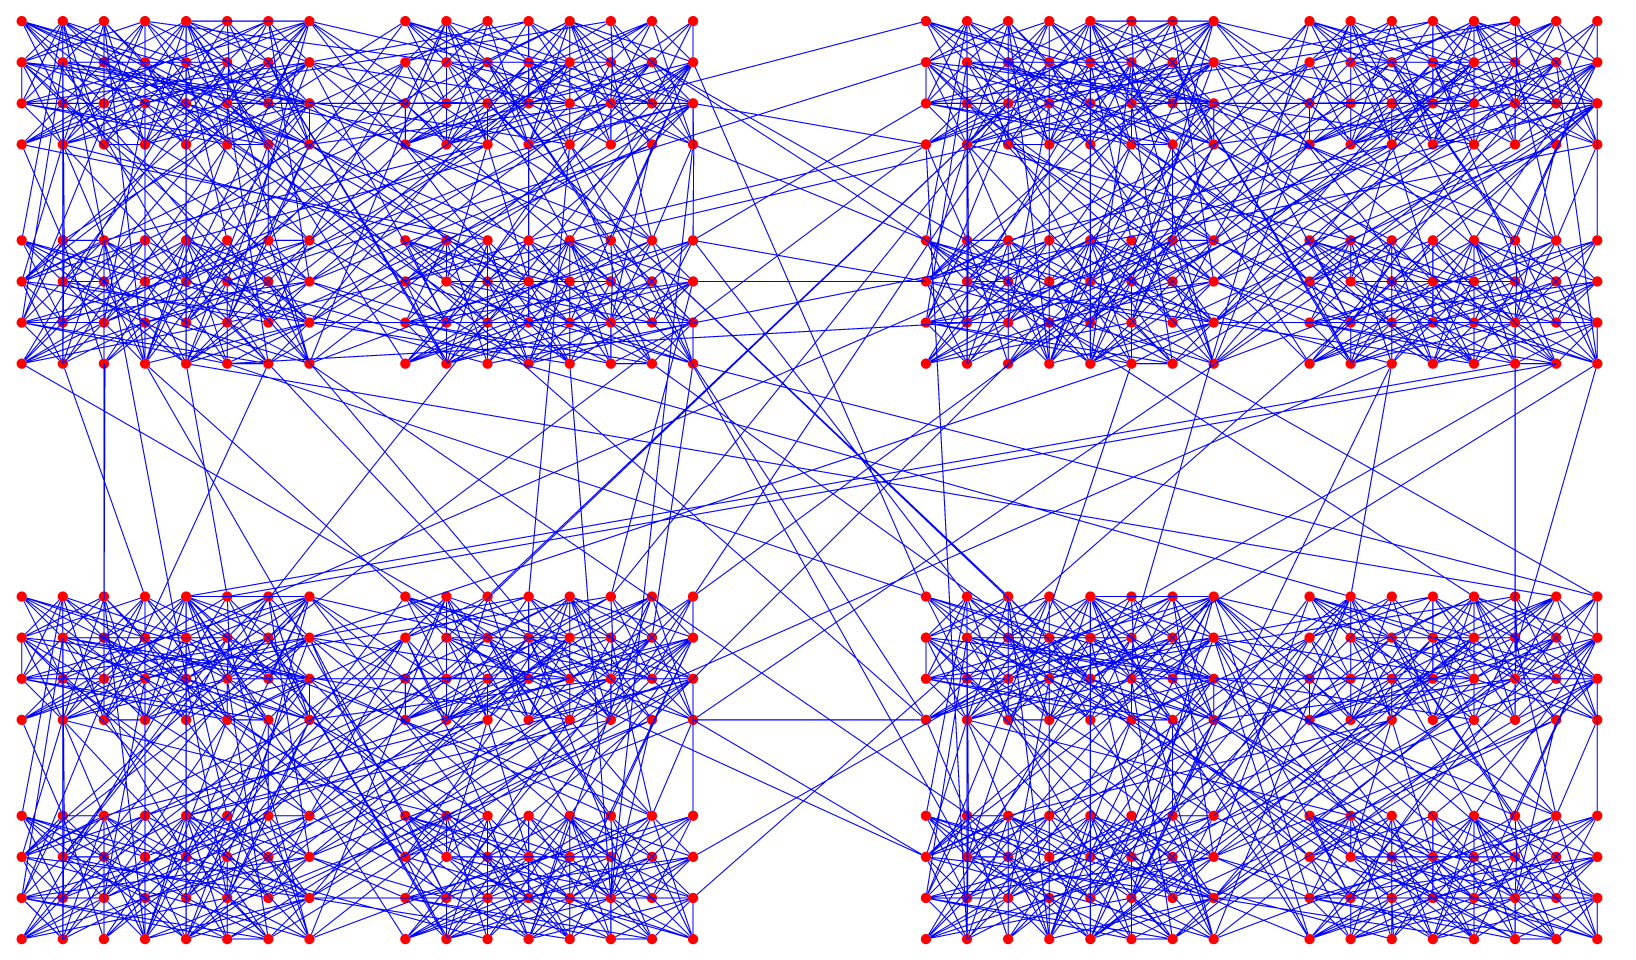
\includegraphics[width=0.8\textwidth]{figures/fortunato2010community_exemplo_comunidades_h.png}}
    \fonte{\citeonline{fortunato2010community}}
\end{figure}

O exemplo da \autoref{fig:graph_hier_com} demonstra como a homofilia as vezes pode ter a presença visualmente verificada.
Considerando que a posição dos vértices na imagem corresponde a duas características ortogonais, a distância entre os vértices pode ser interpretada como uma função de similaridade de dois vértices.
Nesse caso é intuitivamente entendido que vértices mais parecidos se conectam mais do que vértices mais dissemelhantes.

\subsection{Agrupamentos hierárquicos e sobreposições}

No exemplo de grafo da \autoref{fig:graph_hier_com} é possível demonstrar um entendimento intuitivo de como comunidades se organizam.
A estrutura topológica de grupos densamente conectados fica visualmente identificável, onde cada quadrante contém uma comunidade coesa.
Também visualmente acessível, cada comunidade desse exemplo tem uma estrutura interna auto semelhante.

Essa construção de estruturas topológicas recursivas é denominada por \citeonline{girvan2002community} como ``meta grupo'', onde as propriedade topológicas relativas a agrupamentos podem ser encontradas se repetindo em escalas menores dentro das componentes de escalas maiores.
Comunidades podem funcionalmente ser compostas por comunidades menores.
Esse mesmo conceito recebe uma outra nomenclatura nos trabalhos de \citeonline{largeron2015generating, shen2009detect} e \citeonline{fortunato2010community}, onde são descritas como comunidades hierárquicas.

\begin{figure}[htpb]
    \centering
    \caption{Demonstração dos resultados de diferentes algoritmos de detecção em um grafo com comunidades hierárquicas e com sobreposição}\label{fig:graph_hier_over}
    \fbox{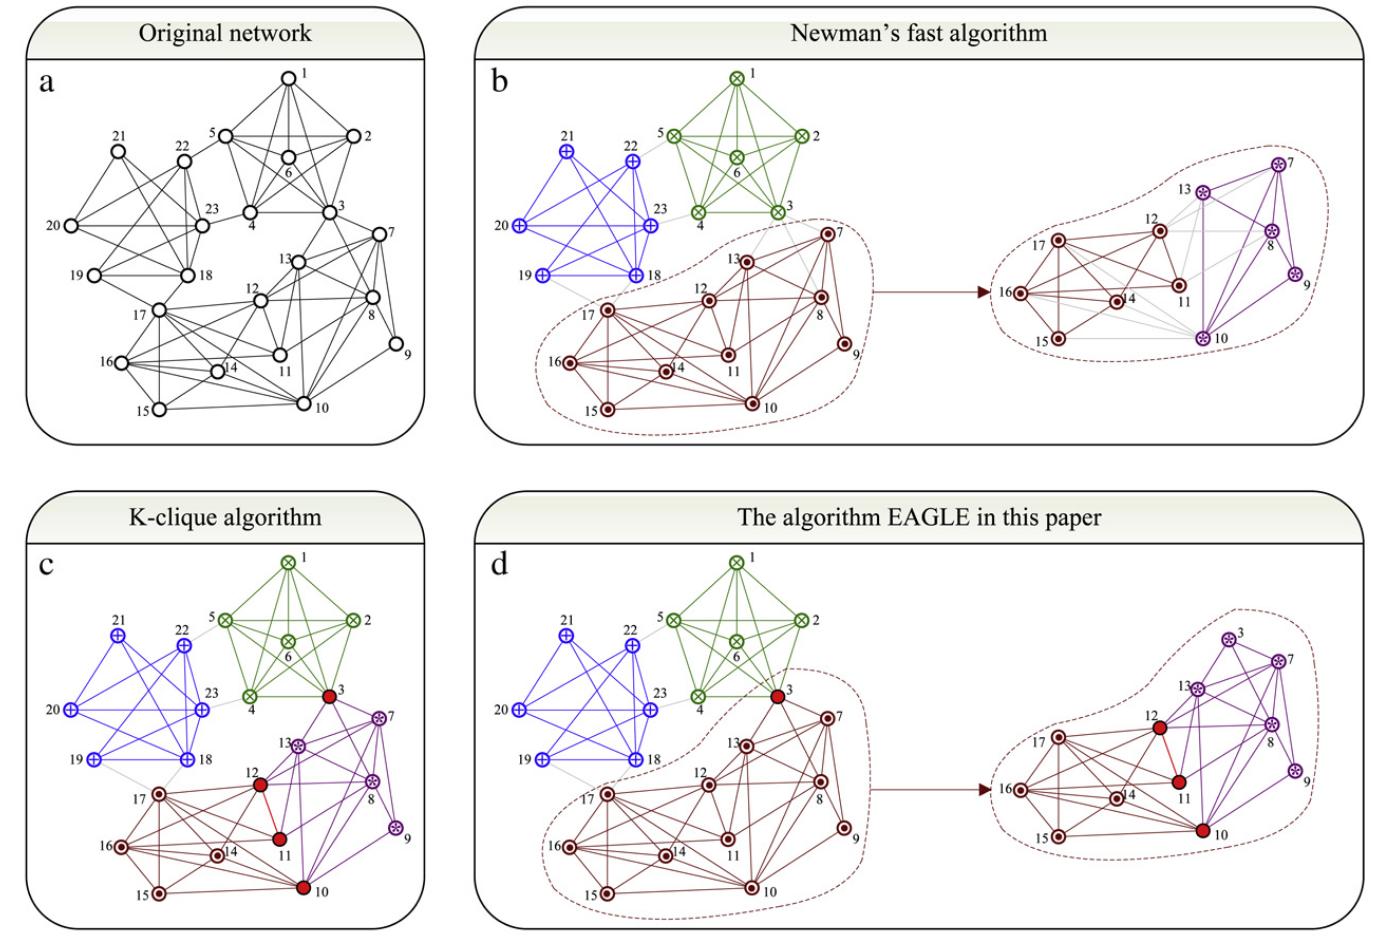
\includegraphics[width=0.8\textwidth]{figures/shen2009detect_graph_com_over.png}}
    \fonte{\citeonline{shen2009detect}.}
\end{figure}

Essas estruturas seguem uma característica recursiva, como demonstrado pelo processo de detecção proposto por \citeonline{shen2009detect}, podendo ser concebidos exemplos de sistemas com qualquer quantidades de níveis.
E a elas também se aplica a compreensão de partição ou cobertura, na \autoref{fig:graph_hier_com} as comunidades de primeiro e de segundo nível caracteristicamente não compartilham vértices.
No caso que demonstram \citeonline{shen2009detect} um vértice pode pertencer a duas somunidades.
Além disso ele pode pertencer a duas comunidades de níveis distintos.
Na \autoref{fig:graph_hier_over}, os resultados de \citeonline{shen2009detect} são demonstrados no quadro a respeito do algoritmo EAGLE, o vértice denotado como 3 é compartilhado entre duas comunidades de primeira ordem, mas em uma delas o vértice 3 encontra-se como membro de uma comunidade de segunda ordem.

Ressaltando que a exata definição de comunidade é altamente dependente do contexto \cite{fortunato2010community}, parece ser consenso na literatura que quando se consideram comunidades hierárquicas, todos os membros de uma comunidade de primeiro nível, devem fazer parte de uma das comunidades que compõe a primeira, como observado nos trabalhos de \citeonline{fortunato2010community} e \citeonline{shen2009detect}.
I.e.: nenhum vértice pertence exclusivamente a uma comunidade sem pertencer a alguma das sub comunidades.
Alternativamente claro, o exemplo da \autoref{fig:graph_hier_over} mostra que a implementação de \citeonline{girvan2002community} (quadrante superior direito) é capaz de produzir partições recursivas (note-se a distinção entre uma cobertura e uma partição).

Essa distinção entre cobertura e grafo implica também na definição de comunidades sobrepostas.
Em sistemas do mundo real que produzem redes complexas, é possível que comunidades compartilhem vértices pois alguma parte de um sistema é componente em dois grupos estruturalmente significantes \cite{shen2009detect}.
Diz-se de duas comunidades que compartilham vértices que elas são comunidades sobrepostas.

O método de detecção de comunidades por K-cliques oferece alguma inspiração no entendimento das propriedades de comunidades sobrepostas.
\citeonline{fortunato2010community} descreve que a forma como esse método trabalha é pivotando subgrafos completos do grafo.
Isso é, dado que um K-clique é um subgrafo completo de $k$ vértices, se dois k-cliques compartilham  $k-1$ vértices, todos os $K+1$ vértices fazem parte de uma mesma comunidade.
Com isso é possível propor que uma cobertura ideal deveria priorizar comunidades com grandes subgrafos completos internamente, mas de que os vértices da intersecção de duas comunidades deveriam participar de k-cliques distintos, preferencialmente não estando adjacentes.
A ideia por trás disso é que se a intersecção de duas comunidades deveria ser parte da periferia das respectivas comunidades \cite{fortunato2010community}.
Se a intersecção fosse tão densamente conexa quando o centro das duas comunidades, esses vértices não seriam mais valores intersectados entre duas comunidades distintas, e as comunidades seriam apenas uma só.

\section{estado da arte\label{sec:estado_arte}}

Existe uma literatura muito prolífica de aplicações dos conceitos de redes complexas, como por exemplo o trabalho de \citeonline{stegehuis2016epidemic}, que fazem uma análise do espalhamento de doenças em uma rede com comunidades, onde é demonstrado que a presença das comunidades tem um efeito significativo.
Muitos métodos para a detecção de comunidades foram propostos, como fica evidente na ampla revisão feita por \citeonline{fortunato2010community}.
Por fim, existe uma literatura também cobrindo diferentes modelos para a geração de redes complexas com comunidades, apesar de bastante mais escassa.

\subsection{RTG: a recursive realistic graph generator using random typing}

\citeonline{akoglu2009rtg} desenvolveram um modelo que gera redes complexas com uma série de proporções que conhecidamente ocorrem em sistemas do mundo real.
Isso é, construindo grafos que se assemelhem aos produzidos pelos sistemas do mundo real.
O modelo também demonstradamente produz grafos com a presença de comunidades.

A implementação realizada por \citeonline{akoglu2009rtg} se baseia em um gerador de arestas que tem as probabilidades tendenciosas.
Esse gerador é o que os autores chamam de um teclado recursivo, na realidade é uma matriz de possibilidades de escolha de uma característica discreta para a origem e o destino em simultâneo.
Nominalmente, os vértices são uma sequência aleatória de caracteres de um conjunto finito de possibilidades, é repetidamente escolhido uma letra para o destino e uma para a origem simultaneamente.
Com um parâmetro controlando um reforço que é feito para que a célula da matriz escolhida a cada interação seja da diagonal principal, existe uma tendência de que vértices adjacentes tenham as mesmas letras nas mesmas posições.

Essas regras simples são o bastante para que o modelo de \citeonline{akoglu2009rtg} tenha como emergentes algumas das propriedades desejáveis em um modelo de geração de redes complexas.
Além das proporções, mundo pequeno, anexação preferencial e homofilia, o sistema de \citeonline{akoglu2009rtg} gera comunidades homogêneas.

Existe também um interesse relevante em quanto os algoritmos de geração de redes complexas precisam em tempo.
Nesse quesito, a implementação de \citeonline{akoglu2009rtg} apresenta algumas das características mais desejáveis, ele é totalmente paralelizável, significando que para a construção de um grafo com o dobro de arestas, é possível dobrar a quantidade de recursos de processamento e assim dobrar a quantidade de arestas produzidas em um tempo constante.

\subsection{Generating Attributed Networks with Communities}

\citeonline{largeron2015generating} apresentam um modelo algorítmico de geração de redes complexas com explícita e deliberada para quais condicionantes são utilizadas para afetar quais propriedades.
Para isso, em uma fase inicial, gera-se uma nuvem de pontos com uma distribuição aleatória e uma amostra dessa população é usada para inicializar as comunidades.
Essa amostragem é processada em um algoritmo k-means, gerando os clusters iniciais, e as arestas iniciais são geradas.
Uma segunda fase processa os demais vértices, escolhendo qual a comunidade serão inseridos se baseando na distância euclideana (homofilia), e gerando os vértices baseado na distribuição de graus.
Numa última fase, opcional, é realizada a introdução de novas arestas, essas arestas são escolhidas de forma a fecharem triângulos, para aumentar o coeficiente de clusterização $C$.

Notadamente, a modelagem de grafo utilizada por \citeonline{largeron2015generating} é $\G = (\V, \E, \A)$ onde  $\A$ é um conjunto de atributos dos vértices vértices, de forma que cada $v \in \V$ é um vetor de valores  $v_A$.
A modelagem tem acompanhando o grafo também um conjunto $\Pa$, composto por conjuntos de vértices, isolando assim as partições.
Essa abordagem oferece uma funcionalidade bastante desejável, que é gerar um catálogo de qual vértice pertence a qual comunidade, dessa forma criando um ``ground truth'' contra o qual o desempenho de alguns algoritmos pode ser testado.
Considerando os trabalhos que utilizam análise de redes complexas como \citeonline{stegehuis2016epidemic}, a possibilidade regerar um grafo com características topológicas conhecidas, podendo-se manipular o coeficiente de clusterização por exemplo, existem um conjunto de possíveis análises com relevância acadêmica.
Para muitas dessas análises, as possibilidades de parametrização do modelo de \citeonline{largeron2015generating} parece ser interessante.
É feita também uma discussão de performance por parte de \citeonline{largeron2015generating}, mas é possível fazer algumas críticas a forma como o modelo foi desenhado, que previnem a paralelização do processo de construção dos grafos.

\end{document}
